\documentclass[11pt, oneside]{article}
\usepackage[letterpaper, margin=2cm]{geometry}
\usepackage{MATH566}
%\usepackage{sagetex}

\begin{document}
\noindent \textbf{\Large{Caleb Logemann \\
MATH 566 Discrete Optimization\\
Homework 3
}}

%\lstinputlisting[language=Sage]{03_2.sage}
\begin{enumerate}
    \item % #1
        Show that
        \begin{center}
            $A\v{x} = \v{b}$ has a nonnegative solution iff
            $\forall \v{y} \in \RR^m$ with $\v{y}^T A \ge \v{0}^T$ implies
            $\v{y}^T \v{b} \ge 0$
        \end{center}
        implies
        \begin{center}
            $A\v{x} \le \v{b}$ has a nonnegative solution iff
            $\forall \v{y} \in \RR^m$, $\v{y} \ge \v{0}$ with $\v{y}^T A \ge \v{0}^T$
            implies $\v{y}^T \v{b} \ge 0$.
        \end{center}

    \item % #2 Done
        Some university in Iowa was measuring the loudness of the fan’s
        screaming during the first touchdown of the local team.
        The measurements contain loudness in dB and the number of people at the
        stadium in thousands
        \begin{center}
            \begin{tabular}{*{6}c}
                \toprule
                \# fans & 53 & 55 & 59 & 61.5 & 61.5 \\
                \midrule
                dB     & 90 & 94 & 95 &  100 &  105 \\
                \bottomrule
            \end{tabular}
        \end{center}
        Find a line $y = ax + b$ best fitting the data.
        There are several different notions of best fitting.
        Commonly used is least squares that is minimizing $\sum*{i}{}{\p{ax_i + b - y_i}^2}$.
        But big outliers move the result a lot (and it is troublesome to do it
        using linear programming).
        Use the one that minimizes the sum of differences. That is
        \[
            \sum{i}{}{\abs{a x_i + b - y_i}}
        \]
        Write a linear program that solves the problem and solve if for the
        ``measured'' data.

        The linear program's objective function should minimize the sum of the
        absolute values of the errors.
        However a linear program's objective function must be linear and
        therefore can't contain any absolute values funtions.
        Instead let $\abs{a x_i + b - y_i} \le e_i$. 
        When $\sum*{i}{}{e_i}$ is minimized, then those inequalities become
        equalities.
        Furthermore, $\abs{a x_i + b - y_i} \le e_i$ can be transformed into two
        linear inequalities that can act as constraints for the linear program.
        Those two inequalties are
        \begin{align*}
             e_i &\ge a x_i + b - y_i \\
            -e_i &\le a x_i + b - y_i
        \end{align*}
        Rearranging this inequalites results in
        \begin{align*}
            -e_i + a x_i + b &\le y_i \\
             e_i + a x_i + b &\ge y_i
        \end{align*}
        Thus the linear program becomes
        \[
            \begin{array}{ll@{}ll}
                \min* & \sum*{i}{}{e_i} \\
                \text{s.t.} & -e_i + a x_i + b \le y_i \quad \forall i \\
                            &  e_i + a x_i + b \ge y_i \quad \forall i
            \end{array}
        \]
        There are no restrictions on $a$ or $b$ they can be any real number.
        The values of $e_i$ must be nonnegative, but we do not require a
        specific constraint for that as the other constraints implies this.

        The following implements this linear program for the given data.
        \lstinputlisting[language=Sage]{03_2.sage}

        The out put of the previous code is
        \begin{verbatim}
            Objective Value: 8.70588235294
            a = 1.17647058824
            b = 27.6470588235
            Errors
            u_0 = 0.0
            u_1 = 1.64705882353
            u_2 = 2.05882352941
            u_3 = 0.0
            u_4 = 5.0
        \end{verbatim}

        \begin{center}
            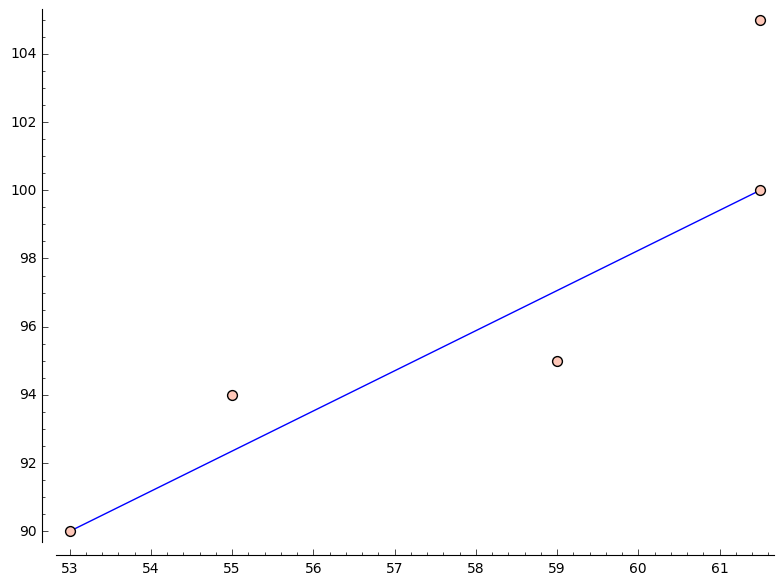
\includegraphics[scale=.5]{Figures/03_1.png}
        \end{center}
        
    \item % #3
        Suppose you are preparing a schedule for classes.
        You have fixed number of classes and students.
        Every student told you which classes (s)he wants to attend.
        However, you do not have enough time slots to run all classes
        sequentially so you need to make some classes run in parallel.
        Create a schedule and argue why it is the best schedule in the sense
        that people as few conflicts as possible.
        You should be able to justify the optimality of the schedule in some sense.
        Make schedule with 3 and with 4 timeslots.
        Assume that there is no limit on how many classes can run in one timeslot.

        Use the following data
        {
        \tiny
            \begin{verbatim}
                [[0,0,0,1,0,1,0,1,0,0,1,0,1,0,0,1,1,1,1,1,1,1,1,0,1,1,1,1,0,0,1,0,0,0,1,1,1,1,1,1,0,1,1,1,1,1,1,0,0,1,0,1,0,0],
                [1,1,1,1,0,1,0,1,0,0,0,1,1,1,0,0,0,0,0,0,1,0,1,0,0,0,0,0,1,1,0,1,0,0,1,0,0,0,1,0,1,0,1,0,0,0,0,1,0,0,1,1,1,0],
                [1,0,1,0,1,0,1,0,1,1,1,1,0,0,1,1,1,1,1,1,0,0,0,1,1,1,0,1,0,0,0,1,0,0,1,1,0,1,1,1,0,1,1,1,1,1,0,0,0,1,1,0,0,0],
                [0,0,1,0,0,0,1,0,0,1,1,0,0,0,0,1,0,0,0,0,0,0,0,0,1,1,0,0,0,1,0,0,1,0,0,0,1,0,0,0,0,0,0,0,1,1,1,0,1,1,0,0,0,0],
                [1,0,0,1,0,1,0,0,0,1,0,0,1,0,0,0,0,0,0,0,0,1,0,1,0,0,1,0,1,0,1,1,0,1,0,0,0,0,0,0,0,0,0,0,0,0,0,0,1,0,0,0,1,0],
                [0,1,1,1,1,0,0,0,1,1,1,1,1,0,1,0,1,1,0,1,0,0,0,0,0,1,0,0,0,1,1,0,0,1,1,0,1,1,1,1,0,0,0,1,1,1,1,0,0,1,0,1,0,1],
                [0,0,1,1,0,1,1,0,0,1,1,1,0,1,1,0,1,1,0,1,0,1,1,0,0,1,1,0,0,0,1,0,0,0,0,0,0,1,0,0,0,0,1,1,0,1,1,0,0,1,0,1,1,0],
                [1,0,0,0,0,1,1,0,1,0,0,0,0,0,0,0,0,0,1,0,1,0,0,0,0,0,1,1,0,0,0,1,0,0,0,1,0,0,0,0,0,0,1,0,1,0,1,0,1,0,0,0,0,0],
                [0,1,0,0,0,1,1,0,1,0,1,0,0,0,0,1,1,1,0,1,0,1,1,1,1,1,0,0,0,0,1,0,1,0,0,0,1,0,1,1,0,0,1,1,1,0,1,0,0,0,0,1,0,1],
                [1,1,1,1,0,1,0,1,0,0,0,1,1,1,0,0,0,0,0,0,1,0,1,0,0,0,0,0,1,1,0,1,0,0,1,0,0,0,1,0,1,0,1,0,0,0,0,1,0,0,1,1,1,0],
                [1,0,1,0,1,0,1,0,1,1,1,1,0,0,1,1,1,1,1,1,0,0,0,0,1,1,0,1,0,0,0,1,0,0,1,1,0,1,1,1,0,1,1,1,1,1,0,0,0,1,1,0,0,0],
                [0,0,1,0,0,0,1,0,0,1,1,0,0,0,0,1,0,0,0,0,0,0,0,0,1,0,0,0,0,0,0,0,0,0,0,0,1,0,0,0,0,0,0,0,1,1,1,0,1,1,0,0,0,0],
                [1,0,0,1,0,1,0,0,0,1,0,0,1,0,0,0,0,0,0,0,0,1,0,0,0,0,1,0,1,0,1,1,1,0,0,0,0,0,0,0,0,0,0,0,0,0,0,0,1,0,0,0,1,0]]
            \end{verbatim}
        }
        Row corresponds to one class, columns corresponds to one students.
        1 means the student wants to attend the class.

\end{enumerate}
\end{document}
